

\chapter{Security Challenges in Smart Constracts}
\markboth{Title of My Seminar Work}{}
\chaptauthors{Lucas Pelloni and Ile Cepilov}

\Kurzfassung{%
This is the abstract.
It fits pretty much on one page and is definitely not longer.}

\newpage

\minitoc %table of contents

\newpage
%http://blockgeeks.com/guides/what-is-blockchain-technology/
%http://www.investopedia.com/terms/b/blockchain.asp
%https://letstalkpayments.com/an-overview-of-blockchain-technology
% PWC: PAPER DA PRENDERE ASSOLUTAMENTE http://www.pwc.ch/en/2017/pdf/pwc_blockchain_opportunity_for_energy_producers_and_consumers_en.pdf


\section{Blockchain Technology}
%TODO 
\subsection{What is a Blockchain?}
A blockchain is like a distributed database which constantly keeps a list of transaction or records,that have ever been executed, called usually blocks. Every record contains a reference to its predecessor and a timestamp.
Data in a record cannot be changed due to its design. This makes them tampering-proof and a very good source of trust for the near future.
The blockchain works and is maintained by the entire community, which verifies all records and acts like a node of a peer-to-peer network, making the need of a thirty part trust organisation useless.
\subsubsection{Source of Trust}
%http://www.investopedia.com/terms/b/blockchain.asp
%A blockchain is a public ledger of all Bitcoin transactions that have ever been executed. It is constantly growing as "completed" blocks are added to it with a new set of recordings. The blocks are added to the blockchain in a linear, chronological order.
Blockchain will become a global decentralised source of trust.
Everything that is centralized makes it easy to attack because it offers a single point of failure. 
(e.g. Firewall of a website). 
Application built with Bloch chain technlogy do not require  users to trust the developers with personal information or funds. 
\subsubsection{How does a Blockchain work?}
           \begin{figure}[ht]
         \begin{center}
         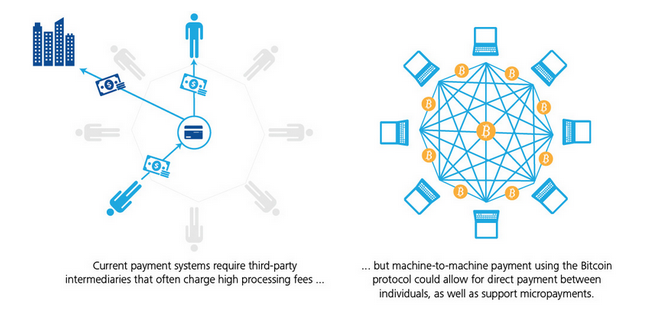
\includegraphics[scale=0.6]{Talk3/blockchain}
         \end{center}
         \caption{This is a pic FROM ILIA}
         \label{label}
       \end{figure}
   
%https://www2.deloitte.com/nl/nl/pages/innovatie/artikelen/blockchain-technology-9-benefits-and-7-challenges.html
\subsection{Benefits of Blockchain Technology}
Every technology that is centralized offers somewhere a point of failure which might be exploited by attackers and nowadays, banks are normally used by most people as a trusted middleman in order to make transaction.
Thanks to its decentralizations, blockchain will avoid the need of a trusted middleman to make transaction by connecting directly buyers and sellers.
%TODO

%http://www.huffingtonpost.com/ameer-rosic-/5-blockchain-applications_b_13279010.html
\subsection{Blockchain applications}
The most famous application of blockchain is in online trades where it gets used for transfering a cryptovalue, bitcoins.
%TODO 


%https://www.shapingtomorrow.com/home/alert/665529-Future-of--Blockchain
%http://usblogs.pwc.com/emerging-technology/the-blockchain-problem-is-a-trust-problem/
\subsection{Future of Blockchain}
%TODO 

%https://www.taylorwessing.com/download/article-how-secure-is-block-chain.html
\subsection{Blockchain security}
%TODO 


\section{Smart Contract: Introduction}
\subsection{Smart Contract: a self-executing contractual agreements}
%definition founded here: https://www.youtube.com/watch?v=FkeLDPZ-v8g&t=134s
A Smart Contract is a piece of software that stores rules for negotiating the terms of a contract, automatically verifies the contract and then executes the agreed terms. 

%https://bitsonblocks.net/2016/02/01/a-gentle-introduction-to-smart-contracts/%
\subsubsection{Traditional vs. Smart Contract}

\subsection{Ethereum: a public blockchain-based platform}
Smart contract applications based on public blockchains.


\subsubsection{Solidity: a typed JavaScript-like language}


\section{Smart Contract attacks}

\subsection{DAO: First Attack}
\subsubsection{Attack description}
\subsubsection{Exploited vulnerability}
\subsubsection{Possible solution}

\subsection{DAO: Second Attack}
\subsubsection{Attack description}
\subsubsection{Exploited vulnerability}
\subsubsection{Possible solution}

\subsection{King of The Ether Throne Attack}
\subsubsection{Attack description}
\subsubsection{Exploited vulnerability}
\subsubsection{Possible solution}

\subsection{MultiPlayer Attack}
\subsubsection{Attack description}
\subsubsection{Exploited vulnerability}
\subsubsection{Possible solution}

\subsection{Rubixi Attack}
\subsubsection{Attack description}
\subsubsection{Exploited vulnerability}
\subsubsection{Possible solution}

\subsection{Govern-Mental: First Attack}
Blablabla said asfbzasfubasbusauhfhu \cite{WinNT}.
\subsubsection{Attack description}
\subsubsection{Exploited vulnerability}
\subsubsection{Possible solution}

\subsection{Govern-Mental: Second Attack}
\subsubsection{Attack description}
\subsubsection{Exploited vulnerability}
\subsubsection{Possible solution}

%http://usblogs.pwc.com/emerging-technology/tag/blockchain/
%http://www.coindesk.com/blockchain-smart-contracts-looming-challenges/
\section{Security Challenges in Smart Contract}
\subsection{No guarantee of transaction execution}
\subsection{Slowness of Smart Contract}
\subsection{Code is slow}



\bibliography{report}{}
\bibliographystyle{plain}
